\section{Stale Synchronous Parallel}

\subsection{Sliding Window Method}
\begin{frame}  
    \frametitle{Sliding Window}
	\begin{itemize}
		\item Sliding Window is an integer range indicating the valid interations.
		\item Clients can not push parameters with the invalid interations. 
		\item Server checks the low bound of the sliding window when the clients push parameters. 
		\item Shift the sliding window. 
	\end{itemize}
\end{frame}


\begin{frame}
    \frametitle{Sliding Window}
	\begin{itemize}
		\item Time complexity
			\begin{itemize}
				\item Clients push parameters: $O(1)$
				\item Server check low bound: $O(1)$
			\end{itemize}
		\item Space complexity: $O(l)$ which l is the length of the sliding window.
			\begin{itemize}
				\item Independent on the \# of clients thus has good scalibility. 
			\end{itemize}
	\end{itemize}
\end{frame}

\subsection{Parallel SGD}
\begin{frame}
    \frametitle{BSP}
    \begin{itemize}
		\item Bulk Synchrnous Parallel
		\item Clients can not continue to the next iteration until the server receives all gradients.
		\item It guarantees converage. 
	\end{itemize}
\end{frame}

\begin{frame}
    \frametitle{ASP}
    \begin{itemize}
		\item Asynchronous Parallel
		\item Clients continue to the next iteration without waiting for each other. 
		\item It may not converage. 
		\item It can be up to 10X slower when the heterogeneity increase.
	\end{itemize}
\end{frame}

\begin{frame}
    \frametitle{SSP}
    \begin{itemize}
		\item Stale Synchrnous Parallel
		\item The faster client can not go ahead the slowest one more than a predefined staleness. 
		\item SGD usually uses this method. 
		\item It can be slower when the heterogeneity increase.
	\end{itemize}
\end{frame}

\begin{frame}
    \frametitle{Constant learning rate, Dynamic learning rate}
    \begin{itemize}
		\item CONSGD
		\begin{itemize}
			\item A constant global learning rate and multiplies it to each local update.
		\end{itemize}
		\item DYNSGC
		\begin{itemize}
			\item To further improve performance over CONSGD.
			\item Server dynamic update global learning rate basing on maximun staleness.
		\end{itemize}
	\end{itemize}
\end{frame}

%\subsection{Server view}
%\begin{frame}
%    \frametitle{Server view}
%    \begin{figure}
%		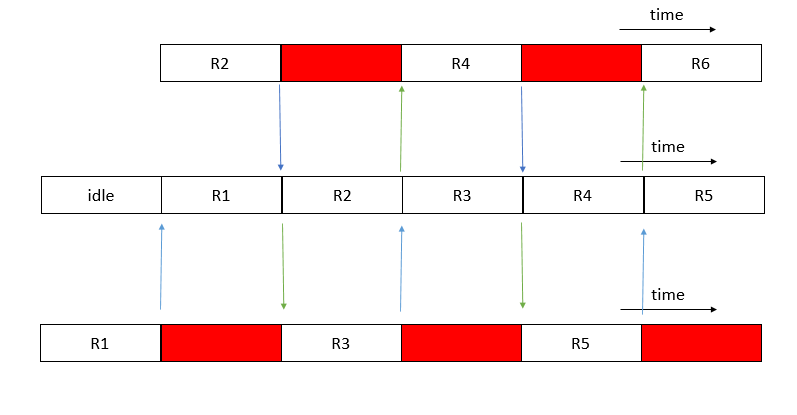
\includegraphics[scale=0.3]{figure/serverview.png}
%	\end{figure}
%\end{frame}



